\documentclass{fkssolpub}

\usepackage[czech]{babel}
\usepackage{fontspec}
\usepackage{fkssugar}
\usepackage{amsmath}
\usepackage{graphicx}

\newcommand{\dd}{\mathrm{d}}
\renewcommand{\angle}{\sphericalangle}

\author{Ondřej Sedláček}
\school{Gymnázium Oty Pavla} 
\series{3}
\problem{A} 

\begin{document}

\begin{figure}[h!]
  \begin{center}
    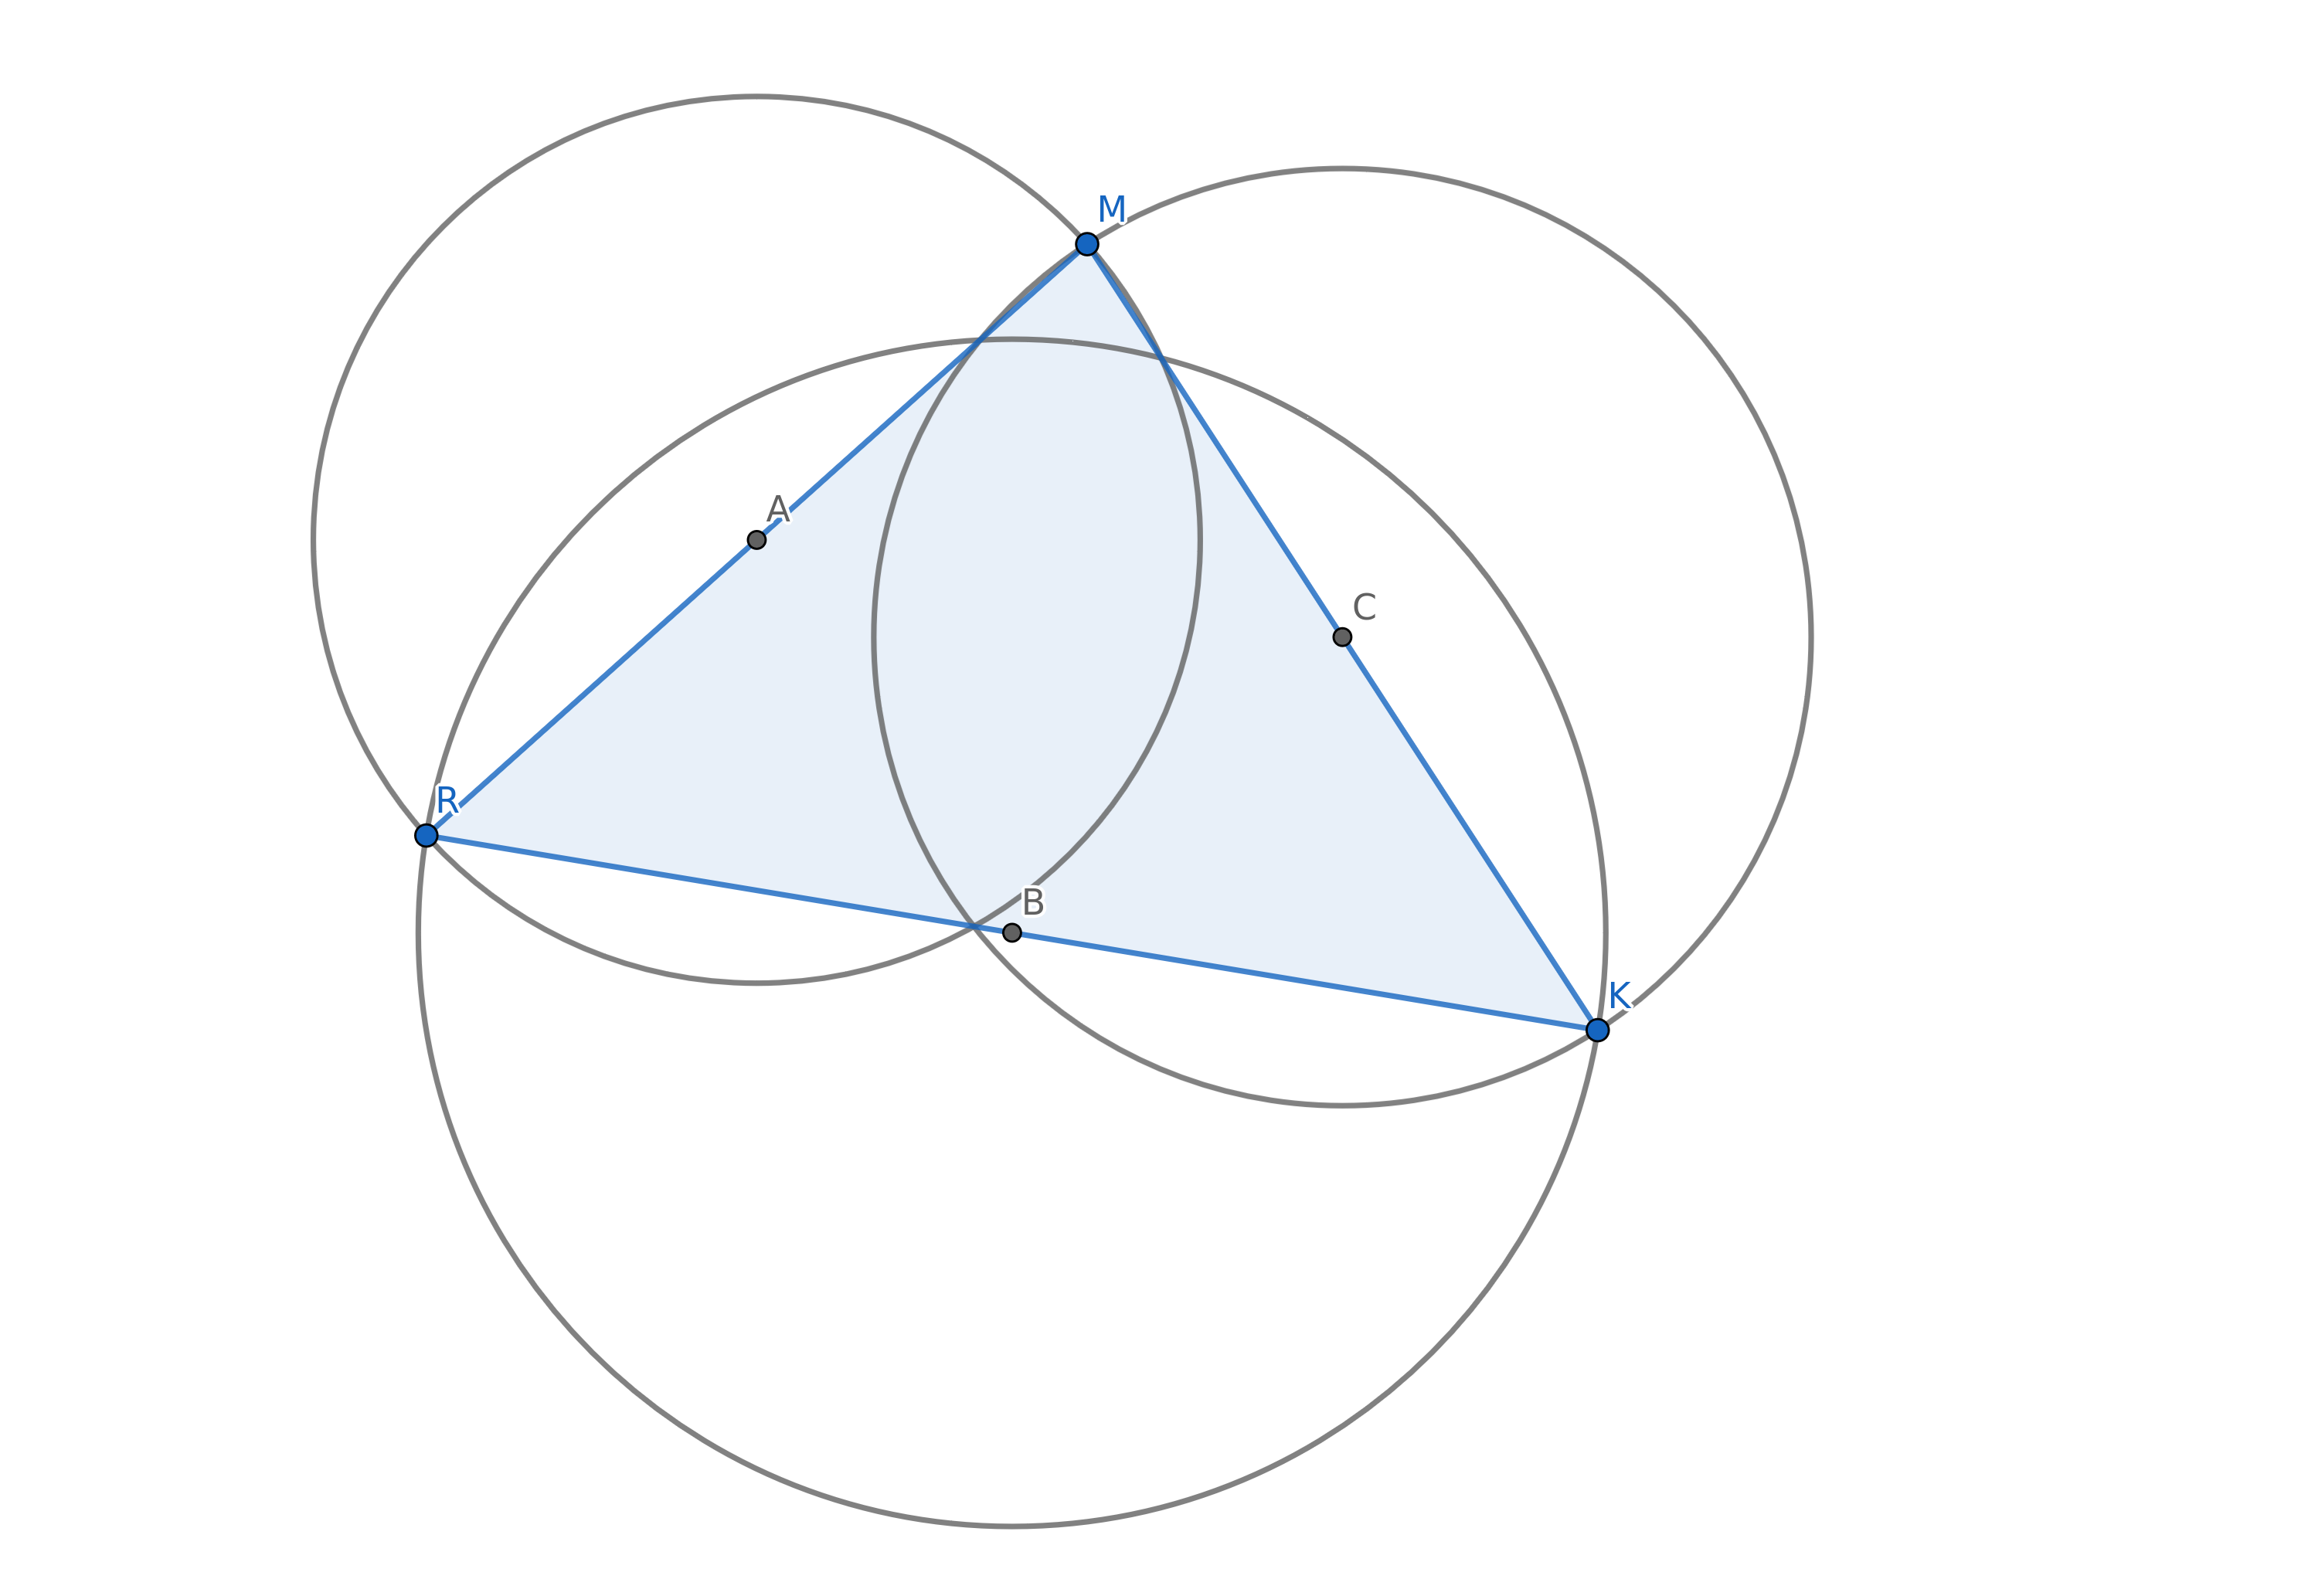
\includegraphics[width=0.95\textwidth]{A-fig.png}
  \end{center}
  \caption{Konstrukce úlohy}\label{fig:}
\end{figure}


Protože tento důkaz je pro každý pár kružnic symetrický, dokážu tento fakt BÚNO pro kružnice nad $MR$ a $RK$. Víme, že každé dvě kružnice se dvěma různými středy může mít nejvýše dva průsečíky. Jeden průsečík již známe -- jedná se o vrchol $R$. A protože $|\angle MRK| < 90^{\circ}$, musí nutně existovat i druhý průsečík, protože pokud by se jen dotýkali, musely by středy a bod dotyku ležet na přímce. 

Nechť tedy označíme druhý průsečík $X$. Ze zadání je zřejmé, že tyto kružnice jsou Thaletovy, a tedy $|\angle MXR| = |\angle RXK| = 90^{\circ}$. Tato vlastnost ale platí také pro patu výšky z bodu $R$, která nutně leží na straně $KM$. A protože žádné další průsečíky nemohou existovat, průsečík $X$ je pata výšky z bodu $R$, která leží na straně $KM$.

Tím je důkaz u konce.

\end{document}
